 \section{Métodos utilizados nesse Estudo e nessa Implementação}

  \begin{frame}{Álgebra Abstrata e de Códigos Corretores de Erros}
     \begin{itemize}
        \item<1-> \emph{Erasure Coding}
        \item<2-> Exame de Qualificação para o Mestrado (EQM)
        \item<3-> Foco: armazenamento de dados
        \item<4-> Códigos corretores de erro disponíveis na versão 0.22  do Hadoop: RAID e RS
    \begin{figure}[hb]
      \centering
      
\includegraphics[scale=2]{hadoop-logo.jpg}
%      \caption{Projeto Hadoop \cite{Hadoop:2010}}
%      \label{fig5:php}
    \end{figure}

        \item<5-> Muitos artigos e material de aulas das disciplinas de universidades de Portugal, Índia, Paquistão e EUA

     \end{itemize}
  \end{frame}

  \begin{frame}{Intuições na Álgebra Abstrata}
     \begin{itemize}
        \item<1-> Congruência linear
        \item<2-> Classes Residuais
        \item<3-> Resto da divisão euclidiana
        \item<4-> Independência linear
        \item<5-> Espaço Vetorial, Grupo, Anel e Corpo (principalmente $\mathbb{GF}_2$ e $\mathbb{GF}_{256}$)
        \item<6-> Sistema de Equações Lineares
        \item<7-> Matrizes
        \item<8-> Polinômios
     \end{itemize}
  \end{frame}

\begin{frame}{Intuições na Álgebra Abstrata}
\begin{definition} {\bf Congruência Linear} \index{Congruência Linear} Seja $q \in \mathbb{Z}$. Dois inteiros $a$
 e $b$ dizem-se congruentes módulo $q$ se, e somente se, $q$ divide $a - b$. A notação é $a \equiv b\,(mod\ q)$. Assim, $a - b\ \in$ $\{x\ tal\ que\ x =  kq, k \in \mathbb{Z}\}$.
\end{definition}

\begin{example}
\begin{align*} % Dois environments aninhados; precisamos arrumar o excesso de espaçamento.
& 32 \equiv 2\,(mod\ 3)\\
& 27 \equiv 5\,(mod\ 11)\\
& 63 \equiv 7\,(mod\ 8)
\end{align*}
\end{example}
  \end{frame}

\begin{frame}{Intuições na Álgebra Abstrata}
\begin{definition} {\bf Conjunto das Classes Residuais} \index{Conjunto das Classes Residuais} Seja $\mathbb{Z}/q = \{\bar{0}_q, \bar{1}_q, \ldots , \overline{q-1}_q\}$ o conjunto das classes residuais dos inteiros módulo $q$. 
\end{definition}

Note que $\mathbb{Z}/q$ tem exatamente $q$ elementos, portanto $\mathbb{Z}/q$ é finito.

As classes residuais possuem propriedades:
  \begin{enumerate}[(i)]
      \item Se a$\ \equiv\ b\,(mod\ q)$, então $\bar{a}_q = \bar{b}_q$.
      \item Se $\bar{a}_q \cap \bar{b}_q  \neq 0$, então $\bar{a}_q = \bar{b}_q$.
      \item Para $a \in \mathbb{Z}, \bigcup \bar{a}_q = \mathbb{Z}$.
  \end{enumerate}

  \end{frame}

  \begin{frame}{Conceitos em Códigos Corretores de Erros}
     \begin{itemize}
        \item<1-> Teoria da codificação $===>$ propriedades dos códigos e suas aplicações
        \item<2-> Teoria da Informação, Claude Shannon~\cite{Shannon:1948} $===>$ incerteza da informação e capacidade do canal
        \item<3-> C. Shannon estudou o processamento digital de sinais (sinais em tempo discreto e em tempo contínuo) em um sistema de comunicação $===>$ hoje, é área da engenharia elétrica e da matemática aplicada
        \item<4-> Sinais podem ser som, áudio, dados biológicos como eletrocardiogramas ou sequências de DNA~\cite{Faria:2010,Faria:2012}, sinais de sistemas de telecomunicações, entre muitos outros.
        \item<5-> Objetivo da codificação de canal é aumentar a resistência do sistema de comunicações digital face aos efeitos do ruído de canal.
     \end{itemize}
  \end{frame}

  \begin{frame}{Conceitos em Códigos Corretores de Erros}
     \begin{itemize}
        \item<1-> Canal binário simétrico
    \begin{figure}[hb]
      \centering
      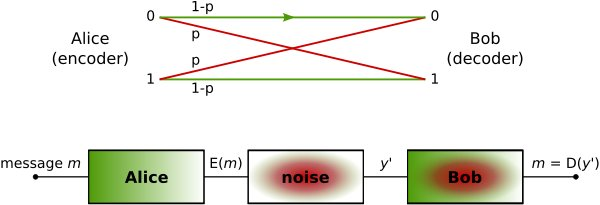
\includegraphics[scale=0.5]{600px-Binary_symmetric_channel.jpg}
%      \caption{Projeto Hadoop \cite{Hadoop:2010}}
%      \label{fig5:php}
    \end{figure}
     \end{itemize}
  \end{frame}

  \begin{frame}{Conceitos em Códigos Corretores de Erros}
     \begin{itemize}
        \item<1-> A ciclicidade de códigos sob anéis comutativos está associada à multiplicação do polinômio gerador pelos diferentes potências de "x" reduzida módulo um polinômio irredutível.
     \end{itemize}
  \end{frame}

  \begin{frame}{Conceitos em Códigos Corretores de Erros}
     \begin{itemize}
        \item<1-> Detectar erros e codificar dados tem a mesma complexidade 
        \item<2-> Decodificar é np-completo
        \item<3-> Estruturas algébricas: matrizes
     \end{itemize}
  \end{frame}

  \begin{frame}{Conhecer e Compilar o código fonte disponível}
   \begin{figure}[hb]
     \centering
     
\includegraphics[scale=0.3]{facebook-logo.jpg}
     
\includegraphics[scale=0.2]{yahoo-logo-300x224.jpg}
     
\includegraphics[scale=0.2]{asf-logo.jpg}
%     \caption{Facebook www.facebook.com}
     \label{fig11:fb}
   \end{figure}
     \begin{itemize}
        \item<1-> Facebook, Yahoo, Fundação Apache
        \item<2-> O \emph{kernel} do Hadoop é constituído do core, hdfs e mapred.
        \item<3-> As versões oficiais para instalação (http://www.apache.org/dist/hadoop/core/) e
        \item<4-> as versões do código fonte (common, hdfs, mapreduce) estão disponíveis em repositório SVN (https://svn.apache.org/repos/asf/hadoop/common/branches/branch-0.22) 
        \item<5-> Na atividade \emph{Scripts for building Hadoop 0.22.0 release}  https://issues.apache.org/jira/browse/HADOOP-6846, os mantenedores e contribuidores do Hadoop discutiam como compilar a versão 0.22
     \end{itemize}
  \end{frame}

  \begin{frame}{Conhecer e Compilar o código fonte disponível}
     \begin{itemize}
        \item<1-> Eclipse IDE for Java
        \item<2-> comandos do linux, principalmente, grep, find e editores de texto
        \item<3-> Doxygen para gerar diagramas de herança e de colaboração das classes a partir do código fonte
        \item<4-> Implementar uma aplicação do \emph{framework} do Hadoop: conta-palavras, temperatura máxima, \emph{page rank}
        \item<5-> Fazer uma pequena alteração no código fonte do RaidNode () para escrever uma mensagem no arquivo de log, compilar o código fonte modificado, instalá-lo e testá-lo
     \end{itemize}
  \end{frame}

  \begin{frame}{Conhecer e Compilar o código fonte disponível}
     \begin{itemize}
        \item<1-> Hadoop foi escrito quase que inteiramente em Java: construtores de classe, asserções
        \item<2-> Java: 1o capítulo do livro vermelho do Sedgewick, Algorithms
        \item<3-> Entender a camada RAID para poder extendê-la
        \item<4-> Entender de álgebra abstrata e de uma de suas aplicações: códigos corretores de erros
        \item<5-> Propor os algoritmos dos novos \emph{codecs}: \emph{encode} e \emph{decode}
     \end{itemize}
  \end{frame}

  \begin{frame}{Conhecer e Compilar o código fonte disponível}
     \begin{itemize}
        \item<1-> Ambiente de edição do código fonte das classes
           \begin{itemize}
              \item<2-> Notebook com Ubuntu $8.04$, depois $10.04$, depois $12.04$ ($2GB$ de RAM, \emph{dual-core}, $150MB$ de disco interno, $1.35TB$ de disco externo) 
           \end{itemize}
        \item<3-> Ambiente de compilação do Hadoop versão 0.22
           \begin{itemize}
              \item<4-> Notebook com Ubuntu
              \item<5-> Laboratório da pós-graduação do IC; estação $64$ bits com Fedora
              \item<6-> Instâncias da Amazon EC2 (servidoras virtuais na Nuvem) com Ubuntu $12.10$,  \emph{kernel},  ($613MB$ de RAM, \emph{dual-core}, alguns \emph{gigabytes} de disco)
           \end{itemize}
        \item<7-> Ambiente de instalação do \emph{tarball}
           \begin{itemize}
              \item<8-> Notebook com Ubuntu
              \item<9-> Instâncias da Amazon EC2
           \end{itemize}
     \end{itemize}
  \end{frame}

  \begin{frame}{Testes Iniciais}
     \begin{itemize}
        \item<1-> Notebook com Ubuntu
        \item<2-> Testes funcionais: \emph{encode} e \emph{decode} das novas codificações e correção de erros no código fonte das classes das codificações implementadas por esse trabalho $===>$ linguagem Java.
     \end{itemize}
  \end{frame}

  \begin{frame}{Testes Finais}

     \begin{itemize}
        \item<1-> Instâncias da Amazon EC2 (servidoras virtuais na Nuvem) com Ubuntu $12.10$,  \emph{kernel},  ($613MB$ de RAM, \emph{dual-core}, alguns \emph{gigabytes} de disco)
        \item<2-> AWS Console e Amazon EC2 API tools (ferramentas de linha de comando)
        \item<3-> 3 fases de Testes de Desempenho (coleta de dados) da operação de \emph{encode} e de Injeção de Falhas das operações de \emph{encode} e \emph{decode} das novas codificações
        \item<4-> Primeira fase: preparação do ambiente de teste
        \item<5-> Rede de 4 instâncias: 1 \emph{master/slave} e 3 \emph{slaves}
        \item<6-> Base de dados: imagens ISO  ($+-800MB$ cada uma)
     \end{itemize}
  \end{frame}

  \begin{frame}{Testes Finais}
     \begin{itemize}
        \item<1-> Segunda fase: coleta de dados para medição de desempenho da operações de \emph{encode} e de \emph{decode} para cada codificação:
                  \begin{itemize}
                     \item replicação simples $2X$
                     \item replicação simples $3X$
                     \item $XOR(6,5)$
                     \item $RS(8,5)$
                     \item $Tornado(10,5)$
                     \item $Tornado(20,10)$
                     \item $Turbo-like(10,5)$
                     \item $Turbo-like(20,10)$
                 \end{itemize}
              \item<2-> Rede de 16 instâncias \emph{large}, provavelmente
        \item<2-> Base de dados: imagens ISO
     \end{itemize}
  \end{frame}

  \begin{frame}{Testes Finais}
     \begin{itemize}
        \item<1-> Terceira fase: coleta de dados para medição da injeção de falhas
           \begin{description}
              \item [falha em $1$ réplica]: corromper $1$ réplica de blocos de dados de um arquivo
              \item [falha em $n$ réplicas] corromper $n$ réplicas de blocos de dados de um arquivo
              \item [falha em réplicas e em blocos de dados] corromper $n$ réplicas de blocos de dados e os $k-1$ blocos de dados de um arquivo
            \end{description}
        \item<2-> Rede de 16 instâncias \emph{large}, provavelmente
        \item<3-> Base de dados: imagens ISO
     \end{itemize}
  \end{frame}
